\chapter{Introducción}

\section*{De lo simple a lo complejo}

\setlength{\parindent}{0cm} Durante la formación en Física, es fundamental el uso constante de ecuaciones diferenciales. Particularmente es obligado abordar el tema de los sistemas lineales de ecuaciones diferenciales ordinarias, con el objetivo de explorar en un primer nivel el comportamiento de diversos fenómenos que dependen del tiempo y de las cantidades que intervienen. Este constante ejercicio ayuda al individuo a modelar sistemas que van desde la resolución del oscilador armónico simple hasta cuestiones más complejas como las que se verán en esta tesis.\\
\\
Un sistema lineal de ecuaciones diferenciales ordinarias consiste en una función vectorial $\textbf{G}:\mathbb{R}^n\to\mathbb{R}^n$ lineal y diferenciable tal que cumple 
$\dot{X}=\textbf{G}(X)$\footnote{considerando que $X(t)\in\mathbb{R}^n$}; al ser lineal es oportuno poder expresar el sistema en términos de una multiplicación de una matriz cuadrada $A\in \mathrm{M}_{n}(\mathbb{R})$ por un vector columna que contiene las funciones lineales de $\textbf{G}$ \cite{hirsch2013differential}
\begin{align*}
	\begin{split}
		\dot{x}_1 &= \underbrace{a_{11}x_1(t)+\cdots+a_{1n}x_n(t)}_{g_1(X)}             \\
		\vdots &\qquad \vdots\qquad\qquad\vdots\qquad\quad\vdots  \\
		\dot{x}_n &= \underbrace{a_{n1}x_1(t)+\cdots+a_{nn}x_n(t)}_{g_n(X)}             
	\end{split}	          
	\qquad\ \ \, \Longleftrightarrow
	\begin{split}
		\underbrace{\begin{pmatrix}
				\dot{x}_1\\
				\vdots\\
				\dot{x}_n
		\end{pmatrix}}_{\dot{X}(t)}=\underbrace{\begin{pmatrix}
				a_{11} & \cdots & a_{1n}\\
				\vdots & \ddots & \vdots\\
				a_{n1} & \cdots & a_{nn}
		\end{pmatrix}}_{A}\underbrace{\begin{pmatrix}
				x_1(t)\\
				\vdots\\
				x_n(t)
		\end{pmatrix}}_{X(t)}
	\end{split} 
\end{align*}
Las constantes de la matriz $a_{ij}\in A$ son coeficientes que describen las interacciones del sistema, mismas que serán responsables de su dinámica, es decir, de la manera en que evolucionará el sistema dependiendo del tiempo y de sus condiciones iniciales. Es conveniente poder contar con esta matriz ya que por si sola brinda información relacionada con la estabilidad del sistema sin la necesidad de llegar a su solución analítica. Para ahondar en el tema de la estabilidad es necesario conocer los \textit{puntos fijos} del sistema.
\\
\\
También llamados \textit{puntos de equilibrio} son aquellos en donde la función vectorial $\textbf{G}$ se hace cero, lo que indica que la dinámica del sistema se mantiene constante o simplemente no cambia. Aunque existe una clasificación, éstos se engloban en dos tipos importantes: puntos de equilibrio \textit{estables} e \textit{inestables}. Esto significa que de acuerdo con las condiciones iniciales del sistema, sus soluciones van a converger o diverger de estos \textit{puntos críticos}. Para poder determinar la estabilidad de estos sistemas, únicamente bastará con saber el signo de los valores propios de la matriz $A$ y se sabrá que mientras todos tengan parte real negativa el sistema será estable, de lo contrario será inestable \cite{hirsch2013differential}.\\
\\
Es bien conocido que para sistemas de dos y tres ecuaciones se encuentra disponible el espacio fase, el cual es útil como herramienta didáctica para visualizar como son los diferentes tipos de puntos de equilibrio, así como para visualizar cómo se comportan las soluciones del sistema. Para valores propios reales se tienen las siguientes opciones
	\begin{figure}[h!]
	\centering
	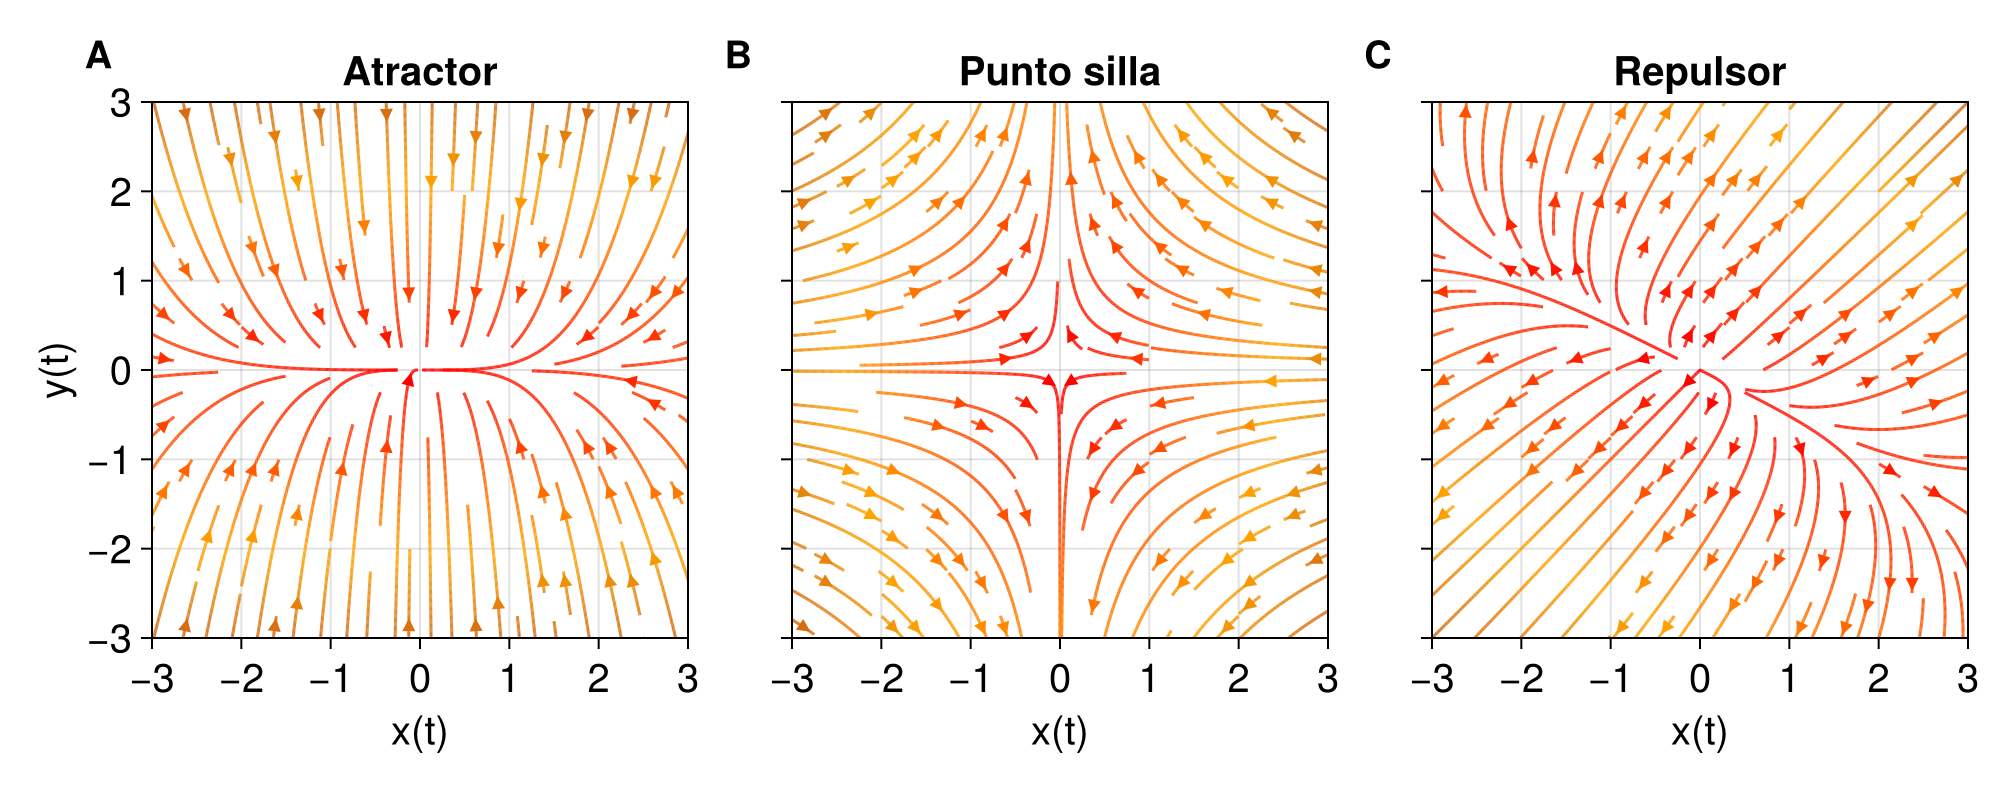
\includegraphics[scale=0.23]{../Imagenes/Espacios fase reales}
	\caption{Espacios fase con valores propios reales.}
	\label{fig:EFReales}
\end{figure}

Y para los valores propios complejos se tienen estas otras opciones.
\begin{figure}[h!]
	\centering
	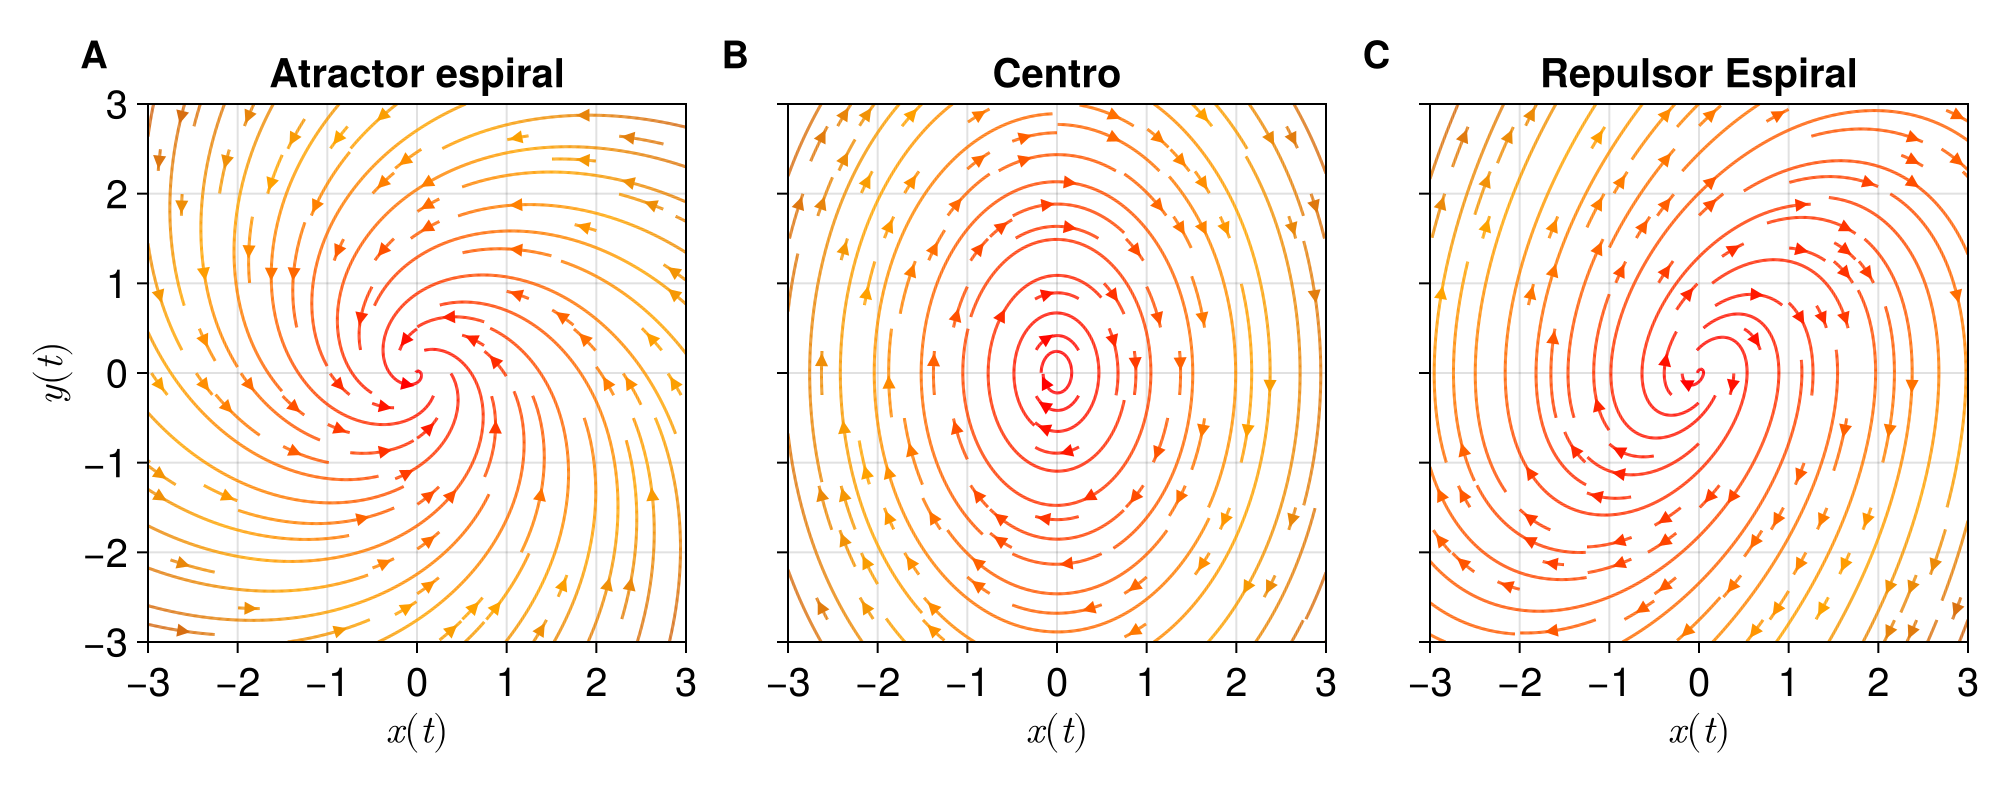
\includegraphics[scale=0.23]{../Imagenes/Espacios fase complejos}
	\caption{Espacios fase con valores propios complejos.}
	\label{fig:EFComplejos}
\end{figure}

Por ahora es importante tener una concepción visual de la dinámica de los sistemas dinámicos lineales, ya que eventualmente se revisarán para $N\gg 1$ en donde es imposible entender la estabilidad en términos de su espacio fase debido a su dimensión. Únicamente atractores (puntos estables), repulsores y puntos silla (puntos intestables) son los que se tomarán en cuenta en esta tesis; los centros se descartarán por completo. Como se ha mencionado, el signo de los valores propios de la matriz a analizar determina la estabilidad del sistema, mientras tengan parte real negativa se puede asegurar que es estable; y si existe al menos un valor propio positivo eventualmente el sistema se hará inestable. Para más detalles de esta clasificación, ahondar en el tercer capítulo de  \cite{hirsch2013differential}.\\
\\
Algo sumamente especial de los sistemas lineales es que cumplen el \textit{principio de superposición} que dicta que una solución y la suma de soluciones del sistema también es solución. Esto implica que los sistemas lineales son simples de describir, pues basta con determinar una sola solución para conocer gran parte de su dinámica. Esto no ocurre del mismo modo con aquellos sistemas que no son lineales y que generalmente son los más interesantes. Como lo dice su nombre, éstos sistemas están constituidos por ecuaciones no lineales que en general no tienen solución única\footnote{Y si la tienen es bajo ciertas condiciones. Ver Teorema de Picard-Lindelöf \cite{CauchyLipschitzTheorem}} o inclusive podrían no tener solución analítica, y aún más complejo si se considera el ensamble de ecuaciones.\\
\\
Gran cantidad de fenómenos en la naturaleza se modelan a partir de sistemas no lineales, y todos ellos comparten la característica de que la suma de sus componentes es mucho más que por sí solas e individuales. La red de neuronas en un cerebro es capaz de generar procesos de donde emerge la consciencia, algo que no puede describir una neurona por sí sola. La gran cantidad de variables que intervienen en el desarrollo y evolución de un huracán es tal que lo hacen realidad, es debido al acoplamiento de éstas que hacen emerger tal fenómeno.\\
\\
En esta ocasión y para esta tesis se estará hablando de poblaciones sin especificar su tipo, se deja al lector la libertad de pensar en los actores protagónicos de estas poblaciones\footnote{Los trabajos en los que se sostiene esta tesis están enfocados en dinámica de poblaciones en el contexto ecológico. Pero esta es solo una interpretación de varias que puedan existir.}. Para hablar de dinámica poblacional conviene recordar un poco sus bases. Teóricamente se comienza a indagar este tema por medio de la siguiente ecuación diferencial
\begin{equation}\label{eqn:CrecimientoExponencial}
	\frac{dP(t)}{dt}=rP(t)
\end{equation}
Lo que representa es la velocidad de crecimiento de una cantidad $P(t)$ que será proporcional a su tamaño actual. El factor de proporcionalidad viene dada por una tasa de crecimiento $r\in\mathbb{R}^+$. Bien se sabe que la solución a esta ecuación es 
$$P(t)=ke^{rt},\qquad\text{con }k\in\mathbb{R}$$
\newpage Aunque se pueda asumir que para cierto periodo el crecimiento de una población puede darse de manera exponencial, la realidad es que ninguna cantidad observable crece de tal forma para cuando $t\to\infty$. Para ello existe una ecuación conocida como \textit{Modelo Logístico} utilizado ampliamente en dinámica poblacional, propagación de enfermedades y sistemas que presenten un crecimiento limitado por recursos
\begin{equation}\label{eqn:EqLogistica}
	\frac{dP}{dt}=rP\left (1-\frac{P}{K}\right )
\end{equation}
este modelo es considerado no lineal por su término cuadrático y es tomado como base para la formación de modelos más elaborados. Tiene un término $K$ que es conocido como la \textit{capacidad de carga} del sistema, y representa el límite de crecimiento que soporta el mismo de modo que las soluciones (independientemente de  la condición inicial que se tome) siempre tienden a esta $K$. Explorando los puntos críticos, el lector podrá comprobar que son para $P_1=0$ y para $P_2=K$, de modo que el primero es un repulsor y el segundo es un atractor. Por medio de líneas fase y series de tiempo es que se puede comprobar lo anterior\footnote{En la sección (\ref{sec:SolEqLogistica}) se puede consultar la solución de la ecuación logística.}
\begin{figure}[h!]
	\centering
	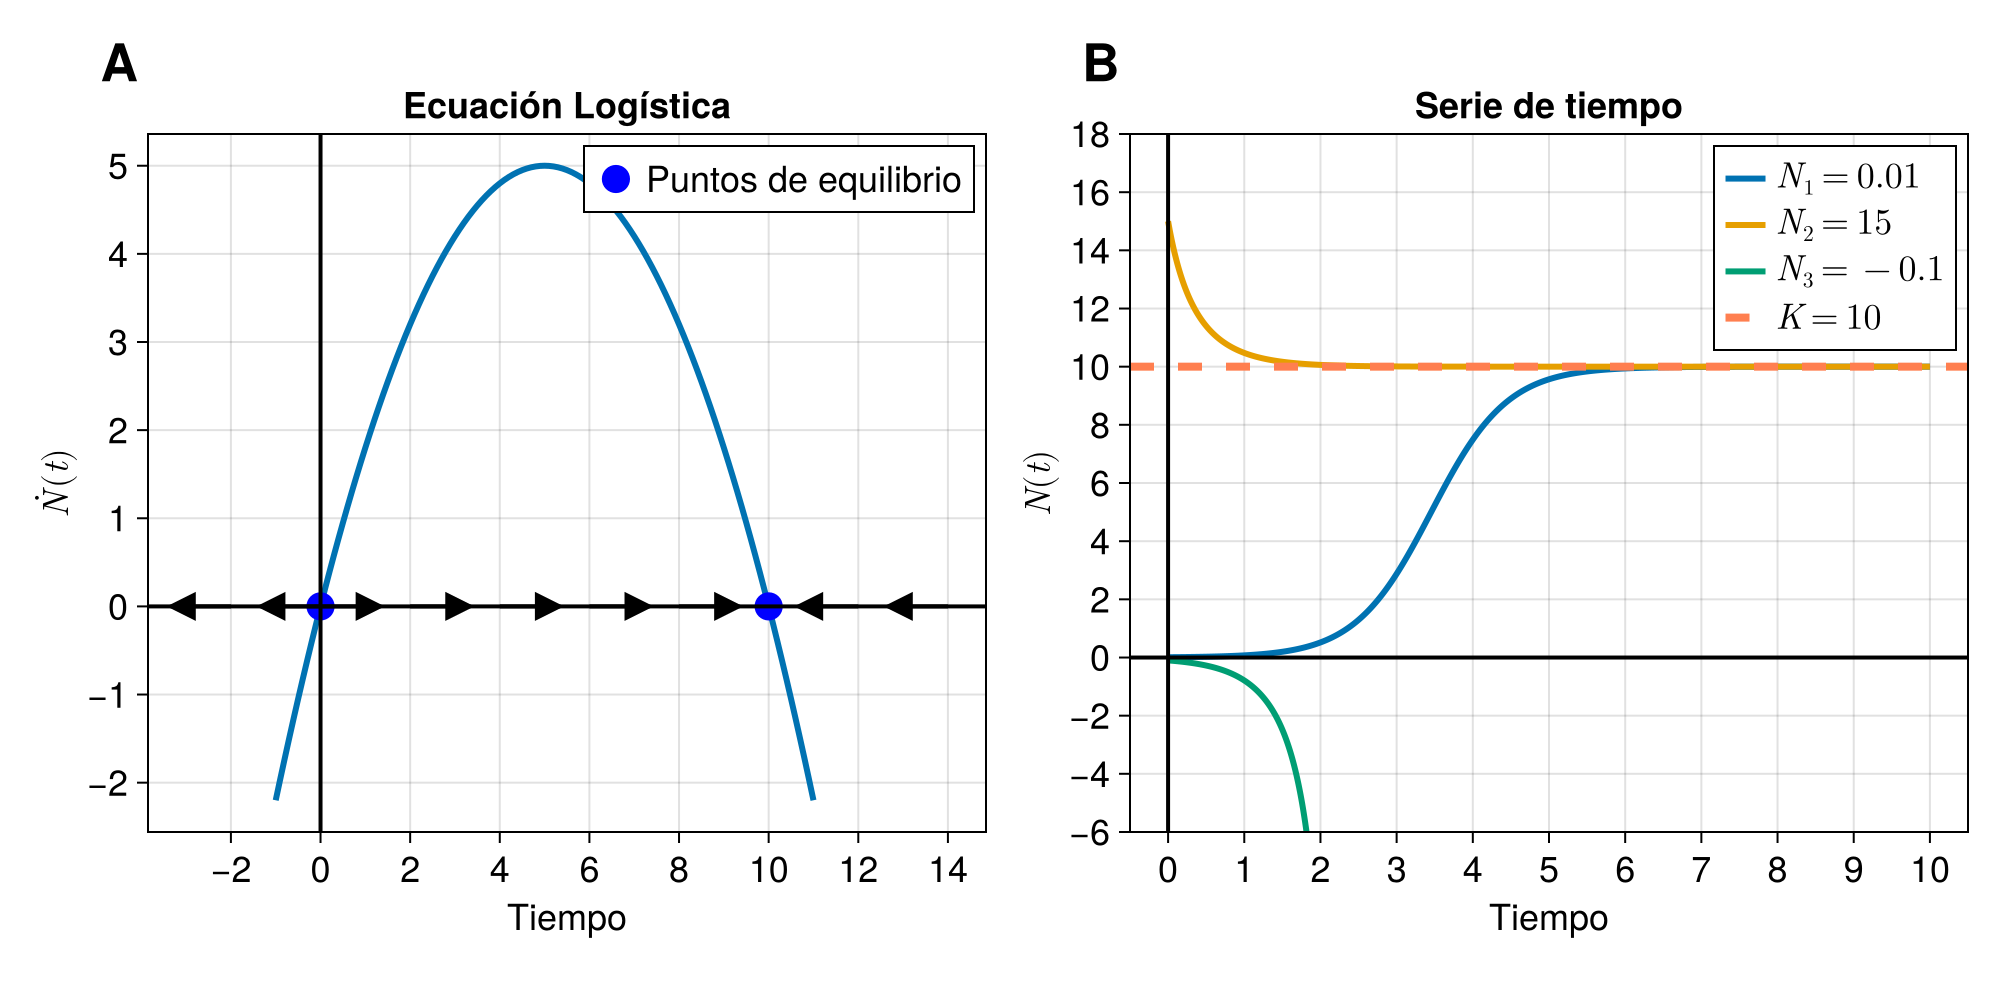
\includegraphics[scale=0.23]{../Imagenes/Ecuacion Logistica}
	\caption{Ecuación logística con una tasa de crecimiento $r=2$ y una capacidad de carga $K=10$. \textbf{A}) Se muestra su linea fase con sus puntos de equilibrio y sus respectivas estabilidades, donde el 0 es repulsor y el 10 es atractor. (\textbf{B}) Solución de la ecuación logística para las condiciones iniciales: $N_1=0.01$, $N_2=15$, y $N_3=-0.1$; se aprecia otra perspectiva de la estabilidad de los puntos fijos.}
	\label{fig:EcuacionLogistica}
\end{figure}		
\newpage
Sin embargo este modelo es para describir la dinámica de una sola población, para poder extender la relación a dos especies y de ahí hasta $N$ se sugieren los modelos de presa-depredador definidos bajo el siguiente sistema
\begin{equation}\label{eqn:PresaDepredador}
	\begin{split}
		\frac{dx}{dt} &= \alpha x - \beta xy\\
		\frac{dy}{dt} &= \delta xy -\gamma y
	\end{split}
\end{equation}

En este sistema $x(t)$ corresponde con la especie de presas y $y(t)$ es la especie depredadora; $\alpha$ corresponde con la tasa de crecimiento de las presas en ausencia de depredadores, $\beta$ es la tasa de depredación y corresponde con la cantidad de presas cazadas, $\delta$ es la tasa de crecimiento de los depredadores a causa del consumo de las presas y $\gamma$ es la tasa de mortalidad de los depredadores en ausencia de presas. La especie presa $x(t)$ crece a diferentes ritmos en el tiempo aún con su tasa de crecimiento $\alpha$ constante, esto debido a que se ve frenada en función de como crecen los depredadores $y(t)$ que van disminuyendo su población. Al mismo tiempo, los depredadores $y(t)$ irán creciendo conforme el número de presas disminuya, pero en algún punto el su cantidad disminuirá tanto que no satisfará la demanda de consumo de los depredadores y por lo tanto esta insuficiencia los hará disminuir\footnote{En la sección (\ref{sec:SolPresaDepredador}) se puede consultar la solución implícita de este sistema.}. \\
\\
Los ritmos de crecimiento de ambas especies vendrá dictada por los coeficientes de interacción y ciertas combinaciones de éstos hace la predominancia de una de las dos especies. En concreto $\beta$ y $\gamma$ ayudan a que las presas predominen en cantidad mientras que $\alpha$ y $\delta$ hacen el mismo papel pero con los depredadores. Para el primer caso $\beta >\alpha$ y $\gamma>\delta$, provoca que exista una alta tasa de depredación con respecto de la natalidad de las presas, significa que hay mucho consumo de presas aún cuando no existan tantas y aunado con el hecho de que se tiene una alta tasa de mortalidad por ausencia de presas hace que disminuya drásticamente el número de depredadores. Esto permite que mientras los depredadores se ven en crisis de población, las presas puedan reproducirse con libertad y sin estar en constante asecho. Finalmente cuando la población de presas se restablece permite que los depredadores también lo hagan y vuelvan a reiniciar el ciclo.
\\
\\
En cambio para que los depredadores puedan predominar en su población solo hay que invertir las desigualdades propuestas y observar que una alta natalidad de presas y un índice de depredación mayor a la mortalidad de los depredadores hace que se mantengan en mayor abundancia que las presas. En la Figura (\ref{fig:SeriesdeTiempoPD}) se aprecian ambos comportamientos antes descritos: Para la gráfica (\textbf{A}) se cumple el primer caso en donde $\alpha<\beta$ y $\delta<\gamma$ y se observa como las presas predominan en población frente a los depredadores mientras que en la gráfica (\textbf{B}) se cumple el segundo caso $\alpha>\beta$ y $\delta>\gamma$ confirmando que los depredadores predominan sobre las presas en su población. \\
\\
Este puede ser uno de múltiples comportamientos, aún pueden existir más combinaciones de los coeficientes que den lugar a otros escenarios. 
\begin{figure}[h!]
	\centering
	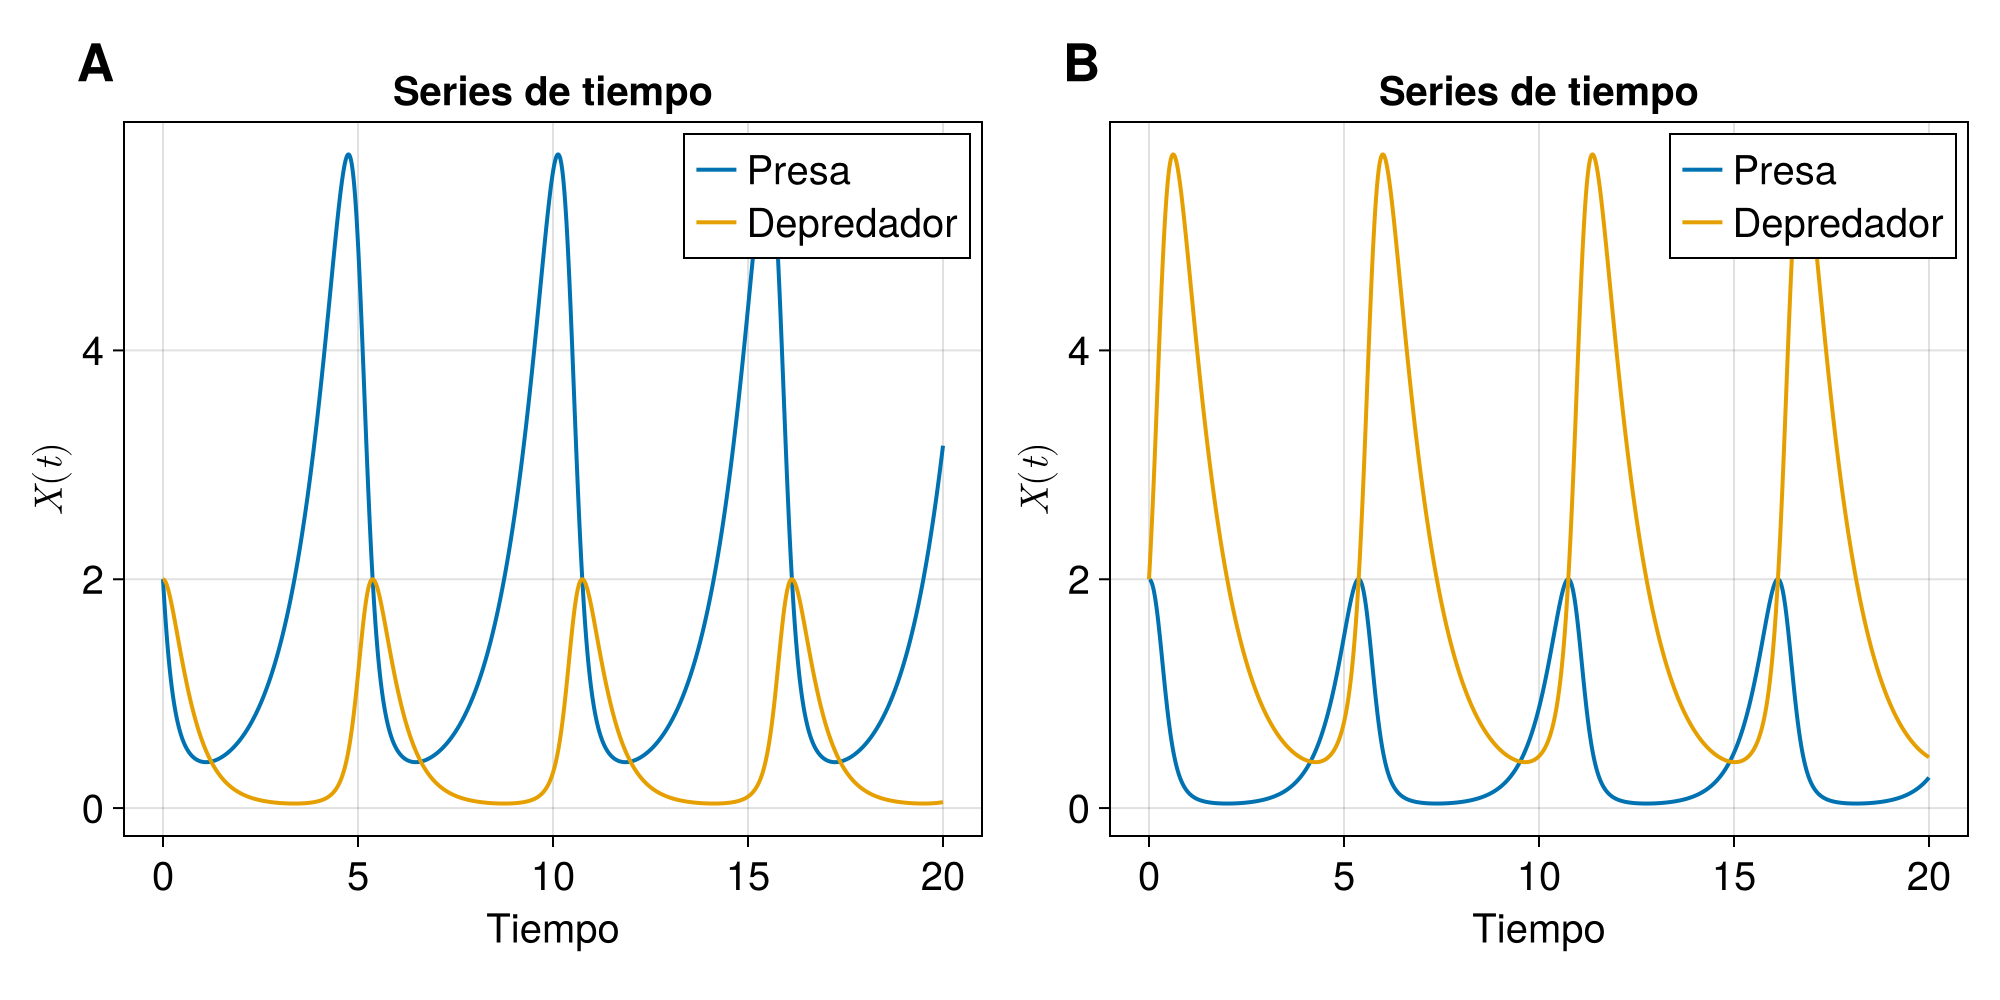
\includegraphics[scale=0.23]{../Imagenes/Series de Tiempo PD}
	\caption{(\textbf{A}) Serie de tiempo del sistema presa-depredador con $\alpha=1$, $\beta=2$, $\gamma=2$ y $\delta=1$. Bajo esta configuración la población de las presas se mantiene predominante sobre la población de depredadores. (\textbf{B}) Serie de tiempo del sistema presa-depredador con $\alpha=2$, $\beta = 1$, $\gamma = 1$ y $\delta = 2$. En este escenario la población de depredadores se mantiene predominante frente a la población de presas.}
	\label{fig:SeriesdeTiempoPD}
\end{figure}

Para una revisión más extensa de este sistema se recomienda consultar el capítulo 8 de \cite{hirsch2013differential}. 
\begin{figure}[h!]
	\centering
	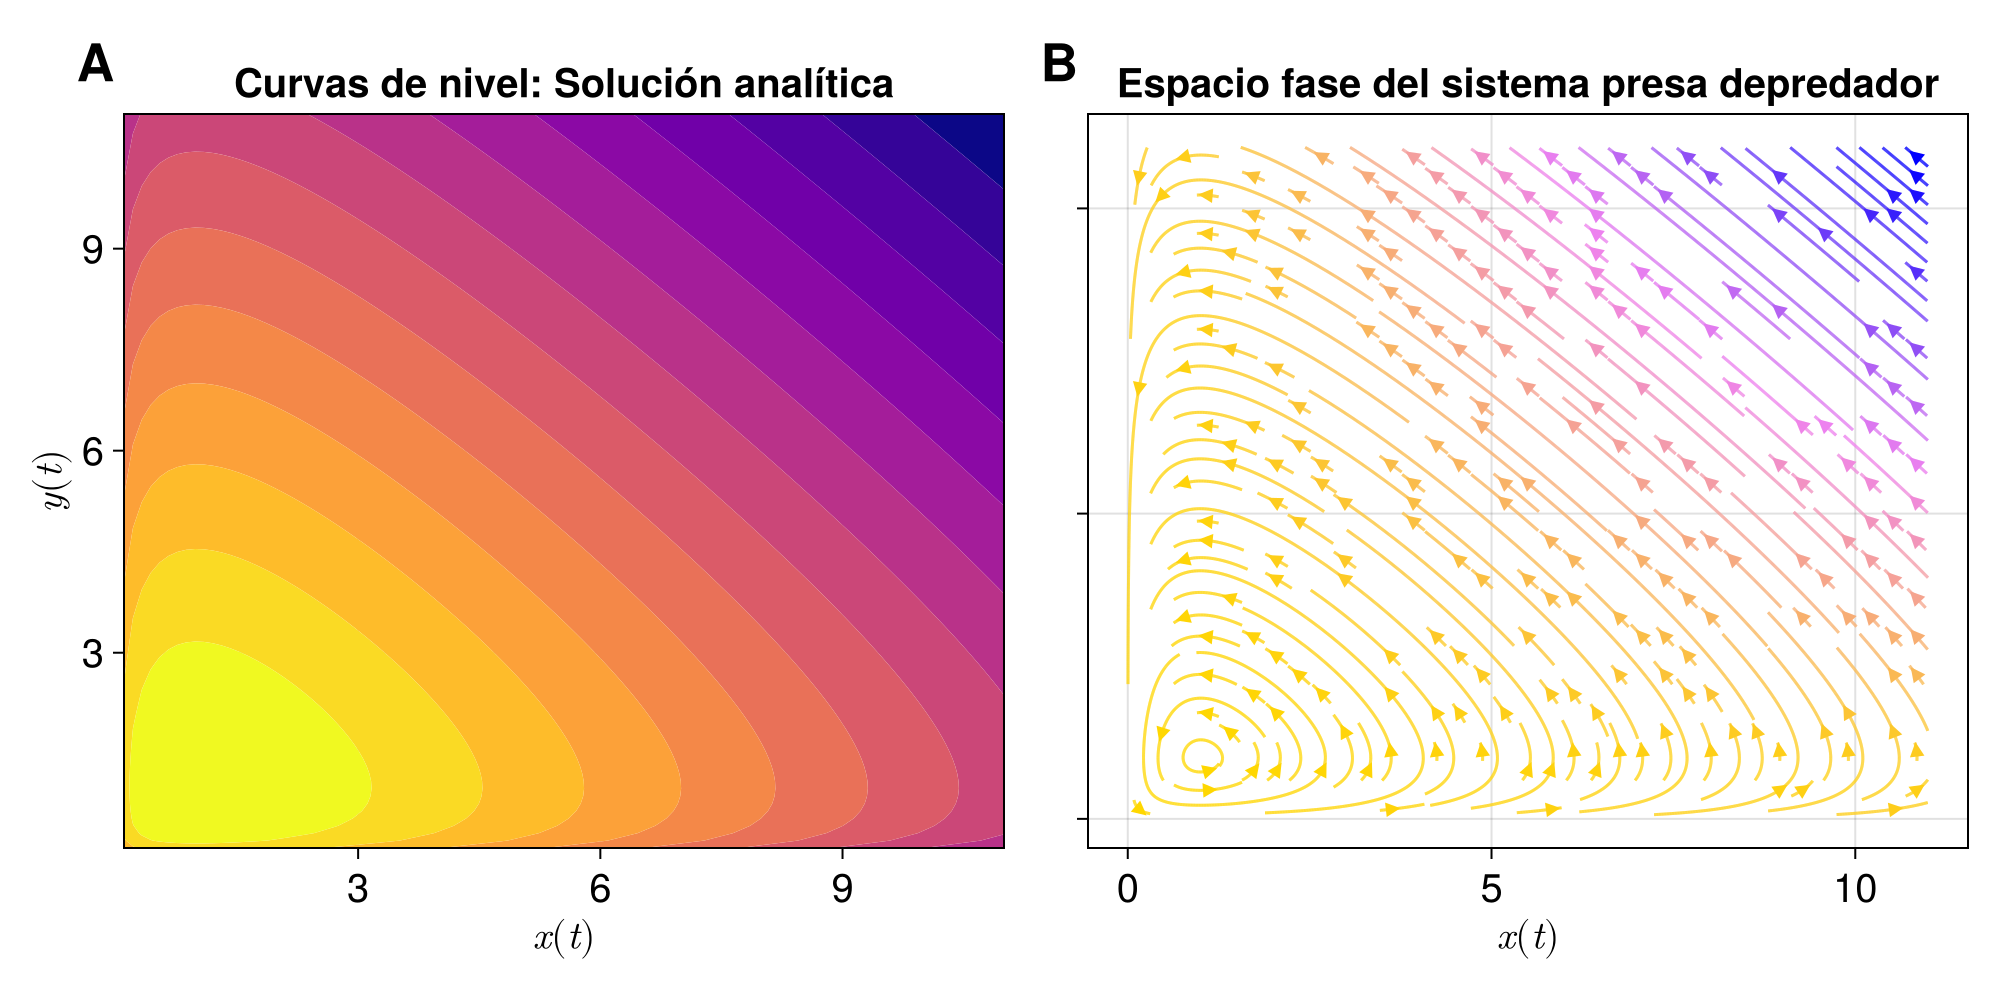
\includegraphics[scale=0.23]{../Imagenes/Curvas de nivel PD}
	\caption{(\textbf{A}) Curvas de nivel utilizando la solución analítica (\ref{eqn:CurvasNivelPD}). (\textbf{B}) Espacio fase generado a partir de las ecuaciones de (\ref{eqn:PresaDepredador}).}
	\label{fig:CurvasNivelPD}
\end{figure}
\newpage
Este breve análisis sobre los coeficientes del sistema ha servido para mostrar su importancia y que prácticamente son los elementos (junto con las condiciones iniciales) que gobiernan la dinámica de los sistemas, pues es la magnitud y configuración de los mismos lo que genera diferentes escenarios de crecimientos (ver Figura (\ref{fig:CurvasNivelPD})).

\subsubsection*{Introducción al modelo especies en competencia}

El sistema de presa-depredador se puede extender al realizar una combinación sutil con la ecuación logística (\ref{eqn:EqLogistica}), es decir, es agregarle una capacidad de carga y la premisa de que ahora no hay especies que depredan y que son depredadas\footnote{Aunque más adelante se verá que si existe una configuración presa-depredador en este sistema.} sino que ahora las especies compiten por los recursos disponibles de un ambiente. Este es el conocido \textit{sistema de competencia de especies} o de Lotka-Volterra de competencia
\begin{equation}\label{eqn:CompentenciaEspecies2x2}
	\begin{split}
		\frac{dx}{dt} &= \alpha x\left (1-\frac{x}{k_1}\right )-\beta xy\\
		\frac{dy}{dt} &= \gamma y\left (1-\frac{y}{k_2}\right )-\delta xy
	\end{split}
\end{equation}
Este sistema de ecuaciones aumenta el número de términos no lineales con respecto del presa depredador, teniendo $x^2$ y $xy$ (para el caso de $\dot{x}$) por lo que también aumenta la complejidad al quererlo resolver de forma analítica\footnote{Si es que tiene solución.}; la solución y análisis de este sistema también se puede hallar en \cite{hirsch2013differential}. A consideración de este autor, esta es la forma más simple de visualizar este sistema. La descripción de ``competencia'' es solamente una de las interacciones posibles del sistema, en el desarrollo de esta tesis se verá que hay otras interacciones posibles que enriquecen la dinámica del sistema y producen escenarios interesantes de analizar.\\
\\
Como es de esperar, la forma de modelar los sistemas y resolverlos será por medio de integración numérica y muchas herramientas computacionales que se irán describiendo en los apéndices/anexos\footnote{Checar esto bien.}. Como método de integración numérica se utilizará \textit{Runge-Kutta} de orden 4 por su precisión; aunque es sabido que el coste computacional es mayor que con otros métodos como Euler, se prefiere asumirlo con tal de tener la mayor precisión posible, pues se sabe que en sistemas no lineales se encuentra muy presente la sensibilidad ante pequeñas perturbaciones, entonces se requiere tener el error mínimo posible.\\
\\
En \cite{stickler2016basic} se pueden consultar la deducción y aplicación de los métodos de Euler y RK4, particularmente las reglas de correspondencia que siguen son 
\begin{equation}\label{eqn:Euler}
	y_{n+1}=y_n+hf(y_n,t_n)+O(h^2)
\end{equation}
para Euler mientras que RK4 obedece la siguiente correspondencia
\begin{equation}\label{eqn:RK4}
	\begin{split}
		Y_1 &= y_n\\
		Y_2 &= y_n+\frac{h}{2}f(Y_1,t_n)\\
		Y_3 &= y_n+\frac{h}{2}f\left (Y_2,t_n+\frac{h}{2}\right )\\
		Y_4 &= y_n+hf\left (Y_3,t_n+\frac{h}{2}\right )\\
		y_{n+1} &= y_n+\frac{h}{6}\left [f(Y_1,t_n)+2f\left (Y_2,t_n+\frac{h}{2}\right)+ 2f\left (Y_3,t_n+\frac{h}{2}\right )+f(Y_4,t_n)\right ]+O(h^5)
	\end{split}
\end{equation}

Para mostrar la diferencia de precisión y la preferencia sobre RK4, se encomienda revisar la Figura (\ref{fig:Rk4vsEuler}) que es una comparación de integrar el sistema (\ref{eqn:PresaDepredador}) con el mismo paso de integración. Para finalizar esta introducción, se ha de mencionar que el trabajo se ha realizado bajo las librerías y lenguaje de programación \julia, por lo que se de invita al lector a emprender un viaje hacia el tratado y análisis de un gran sistema complejo mientras se aprende algo de código en este lenguaje de programación.

 

